\documentclass[a4paper]{article}

\usepackage[margin=2.5cm]{geometry}
\usepackage{graphicx}

\title{Identification of manual control employed during bicycling}

\author{Jason K. Moore, Mont Hubbard, and Ronald Hess}

\date{\today}

\begin{document}

\maketitle

When balancing and directing a bicycle the human rider senses his or her motion
and the environment and then actuates the body to cause the bicycle to travel
in the desired direction. This requires both stabilization, as the
bicycle-rider system is an unstable system, and path following. The most
effective control input for controlling a bicycle under typical operation is to
apply forces to cause the front frame to rotate about the steering axis but
riders are also capable of using body motion to enable control of a bicycle.
It is possible to predict the control actions of the rider using manual control
theory but there have been few attempts to do so while controlling bicycles or
motorcycles.

We have collected a large set of time history data from an instrumented bicycle
which includes the most important kinematic and kinetic variables to describe
the bicycle-rider motion from three different riders on the same bicycle for a
variety of speeds. Furthermore, the instrumented bicycle was designed so that
the riders were not able to move their legs or torso relative to the rear frame
of the bicycle, to ensure that the assumption of rider rigidity of the Whipple
bicycle model was as close to valid as possible and to enforce a single control
input from the rider. In the experiments we perturbed the bicycle-rider system
with an externally applied lateral force and measured the rider's response.

With the single-input multi-output data set in mind we formulate an 8th order
grey box state space model \cite{Ljung1998} in the directly parameterized
innovations form. The model is made up of the plant and the controller. Due to
the poor predictive ability of the Whipple bicycle model we make use of a
bicycle-rider system model identified from a larger superset of the data used
here. We combine this model with a 2nd order model of the rider's neuromuscular
system to form the plant. The controller structure is taken from
\cite{Hess2012} which uses five gains nested in sequential feedback loops each
simulating realistic sensory cues used by the rider.

We then identify the unknown controller gains for each of the runs using the
prediction error method, giving system models that predict the state
trajectories with an average of $62 \pm 12$ percent of the variance accounted
for over all the identified runs, Figure \ref{fig}. The resulting models are
then analyzed and shown to hold well to the manual control theory presented in
\cite{Hess2012}.

\begin{figure}[htb]
  \centering
  % This should be 6 inches wide, but I reduced it to get everything to fit on
  % two pages.
  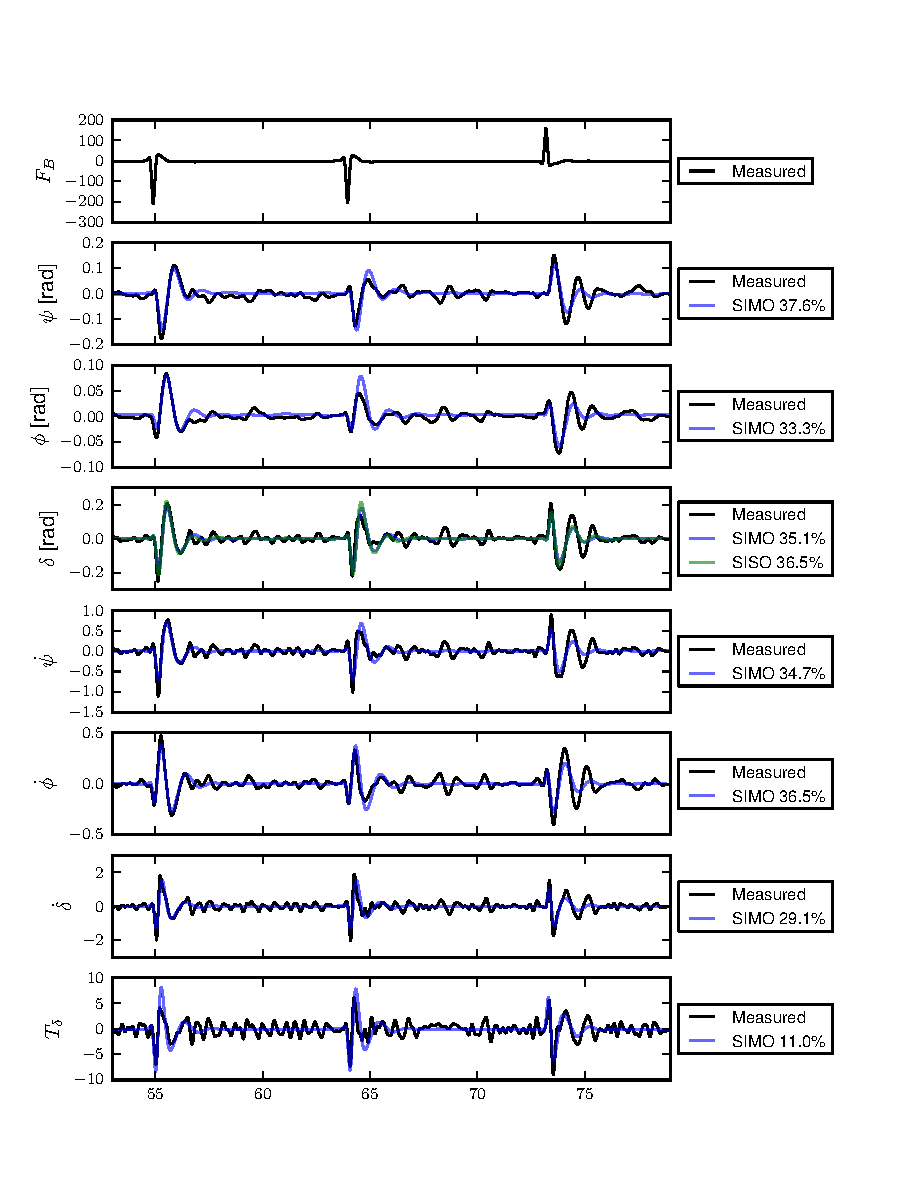
\includegraphics[width=3.85in]{rider-id-treadmill-run.pdf}
  \caption{Simulation of an identified model derived from the inputs and
  outputs (SIMO) of one of Charlie's treadmill runs \#288 (4.23 m/s) validated
  against the data from run \#289 (4.22 m/s). The black line is the processed
  and filtered (low pass 15 Hz) measured data, the blue line is the simulation
  from the identified SIMO model and the green line is the identified SISO
  model.}
  \label{fig}
\end{figure}

We show that a simple rider controller can be identified from the collected
data given that the plant model of the bicycle/rider system is properly chosen.
In addition, these basic conclusions arise: (1) The fundamental, remnant-free,
control response of the rider under lateral perturbations can be described
reasonably well by the simple five gain sequential loop closure and an eighth
order closed loop system. (2) No time delays are needed and the continuous
formulation is adequate for good prediction, (3) The identified gains seem to
exhibit linear trends with respect to speed as predicted by theory and the
identified neuromuscular frequency seems to be constant with a median around
the theoretical prediction of 30 rad/s, (4) The identified parameters show
resemblance to the patterns in the theoretical loop closure techniques,
especially in that the riders select their gains such that the closed roll rate
loop exhibits a 10 dB peak around 10-11 rad/s and the riders cross over the
outer three loops in the predicted order, (5) the crossover frequencies of the
three outer loops are relatively constant with respect to speed and point to a
speed independence of system response bandwidth selection among riders in this
task.

This paper is based on work supported by the National Science Foundation under
Grant No 0928339.

\bibliographystyle{plain}
\bibliography{references}

\end{document}
